

\documentclass{beamer}
\usepackage[super]{nth}

\usetheme{Madrid}

\makeatother
\setbeamertemplate{footline}
{
  \leavevmode%
  \hbox{%
  \begin{beamercolorbox}[wd=.2\paperwidth,ht=2.25ex,dp=1ex,center]{author in head/foot}%
    \usebeamerfont{author in head/foot}\insertshortauthor
  \end{beamercolorbox}%
  \begin{beamercolorbox}[wd=.8\paperwidth,ht=2.25ex,dp=1ex,center]{title in head/foot}%
    \usebeamerfont{title in head/foot}\insertshorttitle\hspace*{3em}
    \insertframenumber{} / \inserttotalframenumber\hspace*{1ex}
  \end{beamercolorbox}}%
  \vskip0pt%
}
\makeatletter
\setbeamertemplate{navigation symbols}{}
\title{PhD Application for The PhD Thesis\\ "Decentralized Fog Computing Infrastructure Control"}


\subtitle{}

\author{Ali J. Fahs}%\\ Supervisor: Professor Guillaume Pierre}



\institute[Institut de Recherche en Informatique et Systèmes Aléatoires (IRISA)] % (optional, but mostly needed)
{
  
  Institut de Recherche en Informatique et Systèmes Aléatoires (IRISA)\\MYRIADS Team\\Supervised by Professor Guillaume Pierre 
  
  
  }

\date{Audition, \nth{8} of June, 2017}

\subject{PhD Application}

\begin{document}

\begin{frame}
  \titlepage
\end{frame}

\begin{frame}{Outline}
  \tableofcontents
 
\end{frame}

%%%%%%%%%%%%%%%%%%%%%%%%%%%%%%%%%%%%%%%
\section{Personal Presentation}
\begin{frame}{Personal Presentation}
\begin{itemize}
\item A double diploma student.
\begin{itemize}
\item Engineering diploma in telecommunication and computer science - Lebanese University, Faculty of engineering (Home University).
\item Master's degree in Informatics Grenoble (MoSIG) Parallel, Distributed Systems Track - Grenoble INP, Ensimag jointly with UGA, IMAG (Host University).
\end{itemize}

\item Research interest: Distributed systems, Networking.
\item Master's thesis "Distributed Approach for Cross-Layer Resource Allocation in Wireless Sensor Networks" Jointly between LIG and VERIMAG.
\end{itemize}

 
\end{frame}


%%%%%%%%%%%%%%%%%%%%%%%%%%%%%%%%%%%%%%%%%%%%%%%%%%%%%
\section{Master Thesis}



\begin{frame}{Master Thesis}

\begin{minipage}[t]{0.48\linewidth}

\begin{block}{Internship objectives}
    \begin{itemize}
    \item Improvement in the distributed 6TiSCH networks
    \item<2-> Reduction of collision in TSCH Dedicated cells.
     \item<3-> The distributed approach causing the problem. 
      \item<4-> Lack of central entity. 
      
     
    
    \end{itemize}
    \end{block}
\end{minipage}\hfill
\begin{minipage}[t]{0.48\linewidth}
\centering
\begin{figure}[p]

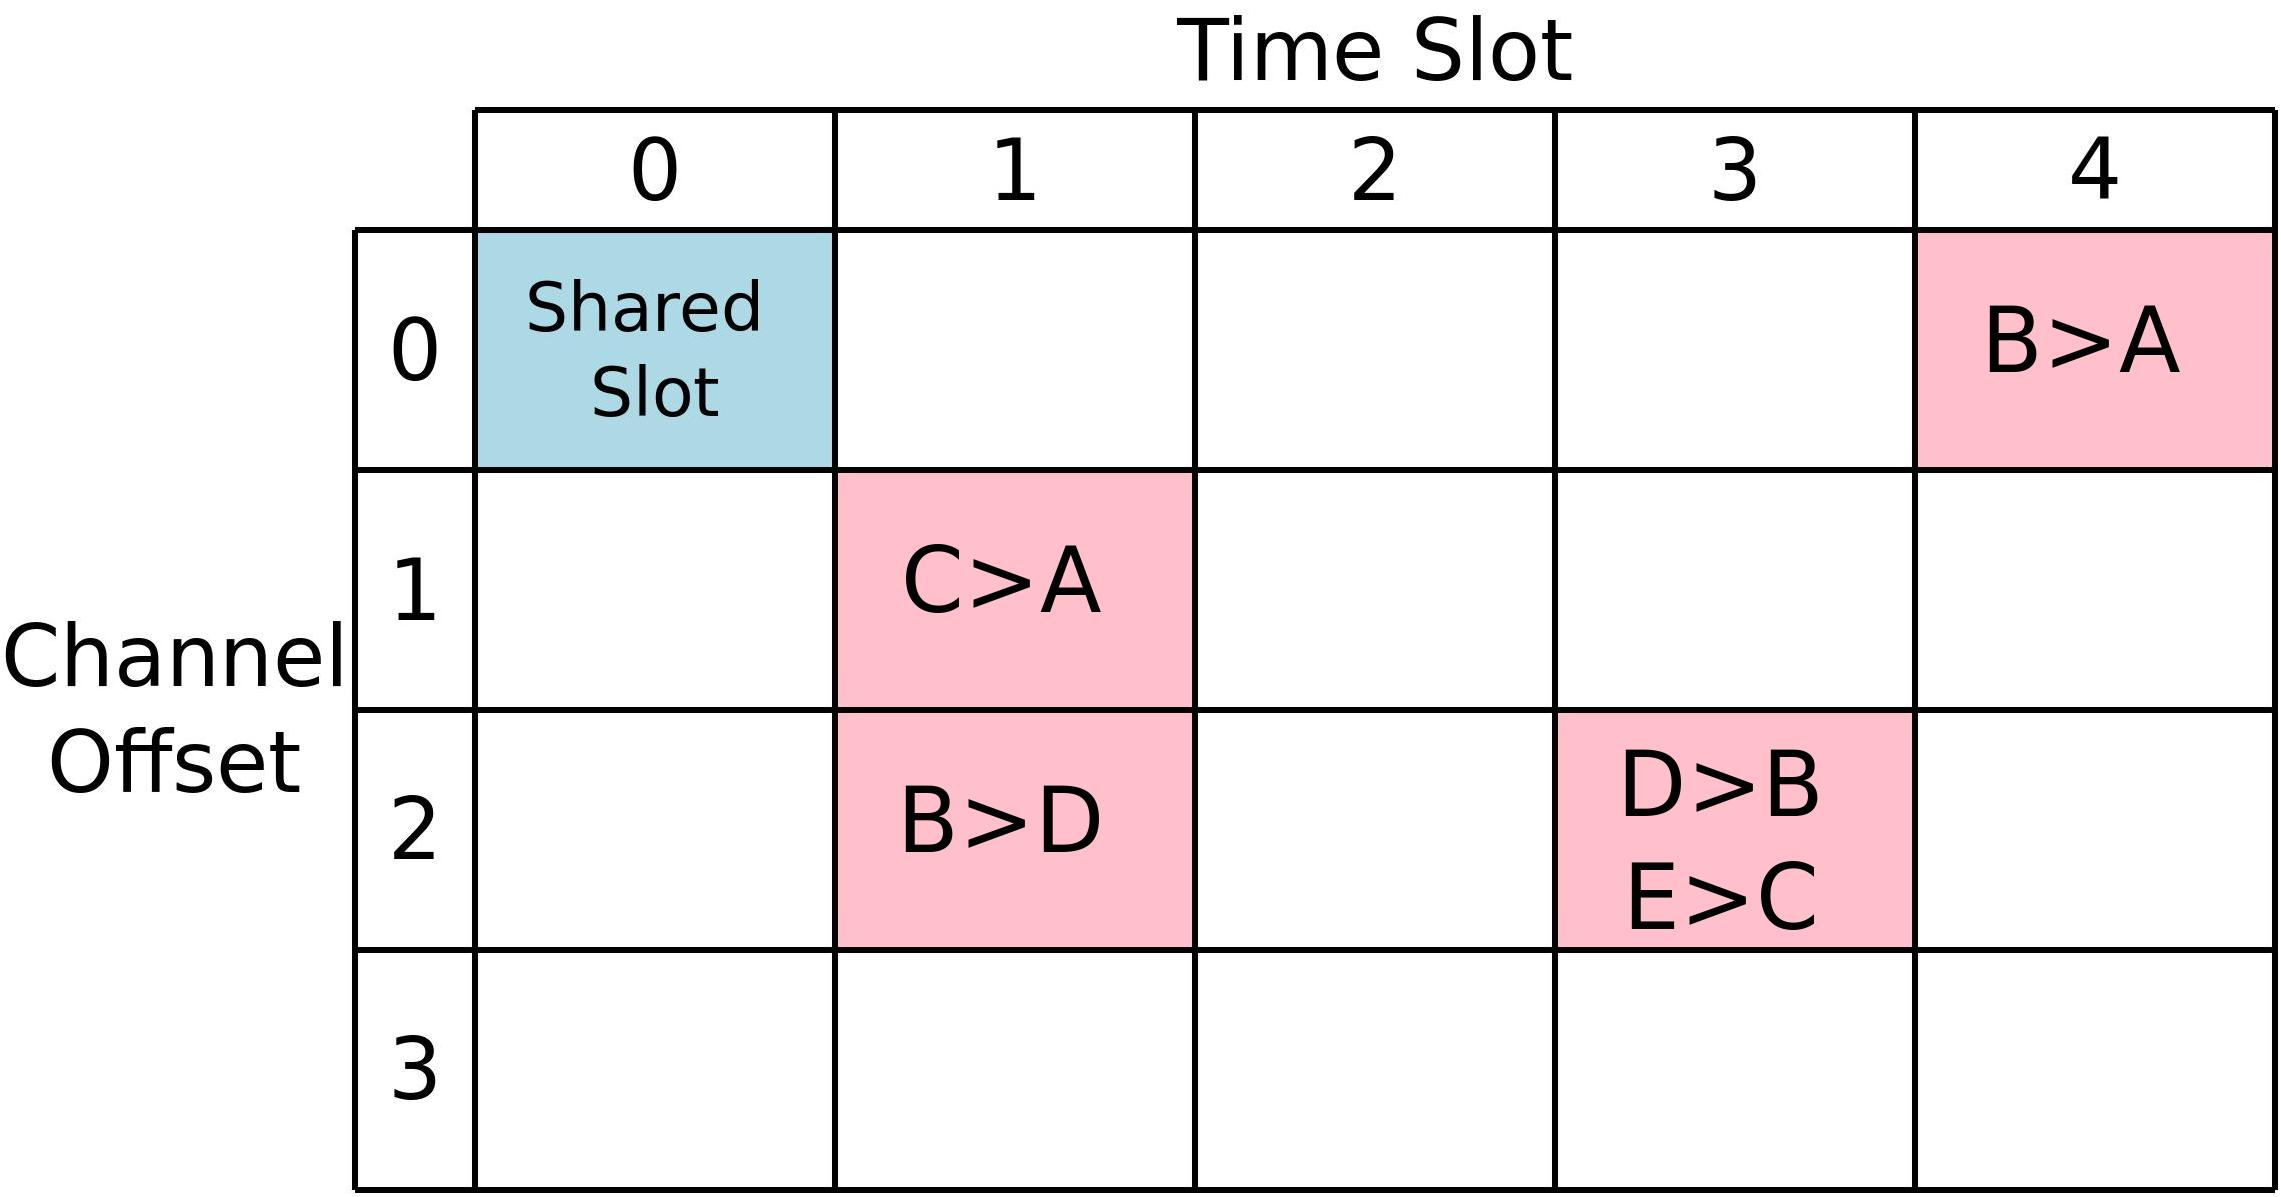
\includegraphics[width=\linewidth]{TSCH.jpeg}

\end{figure}
\begin{figure}[p]


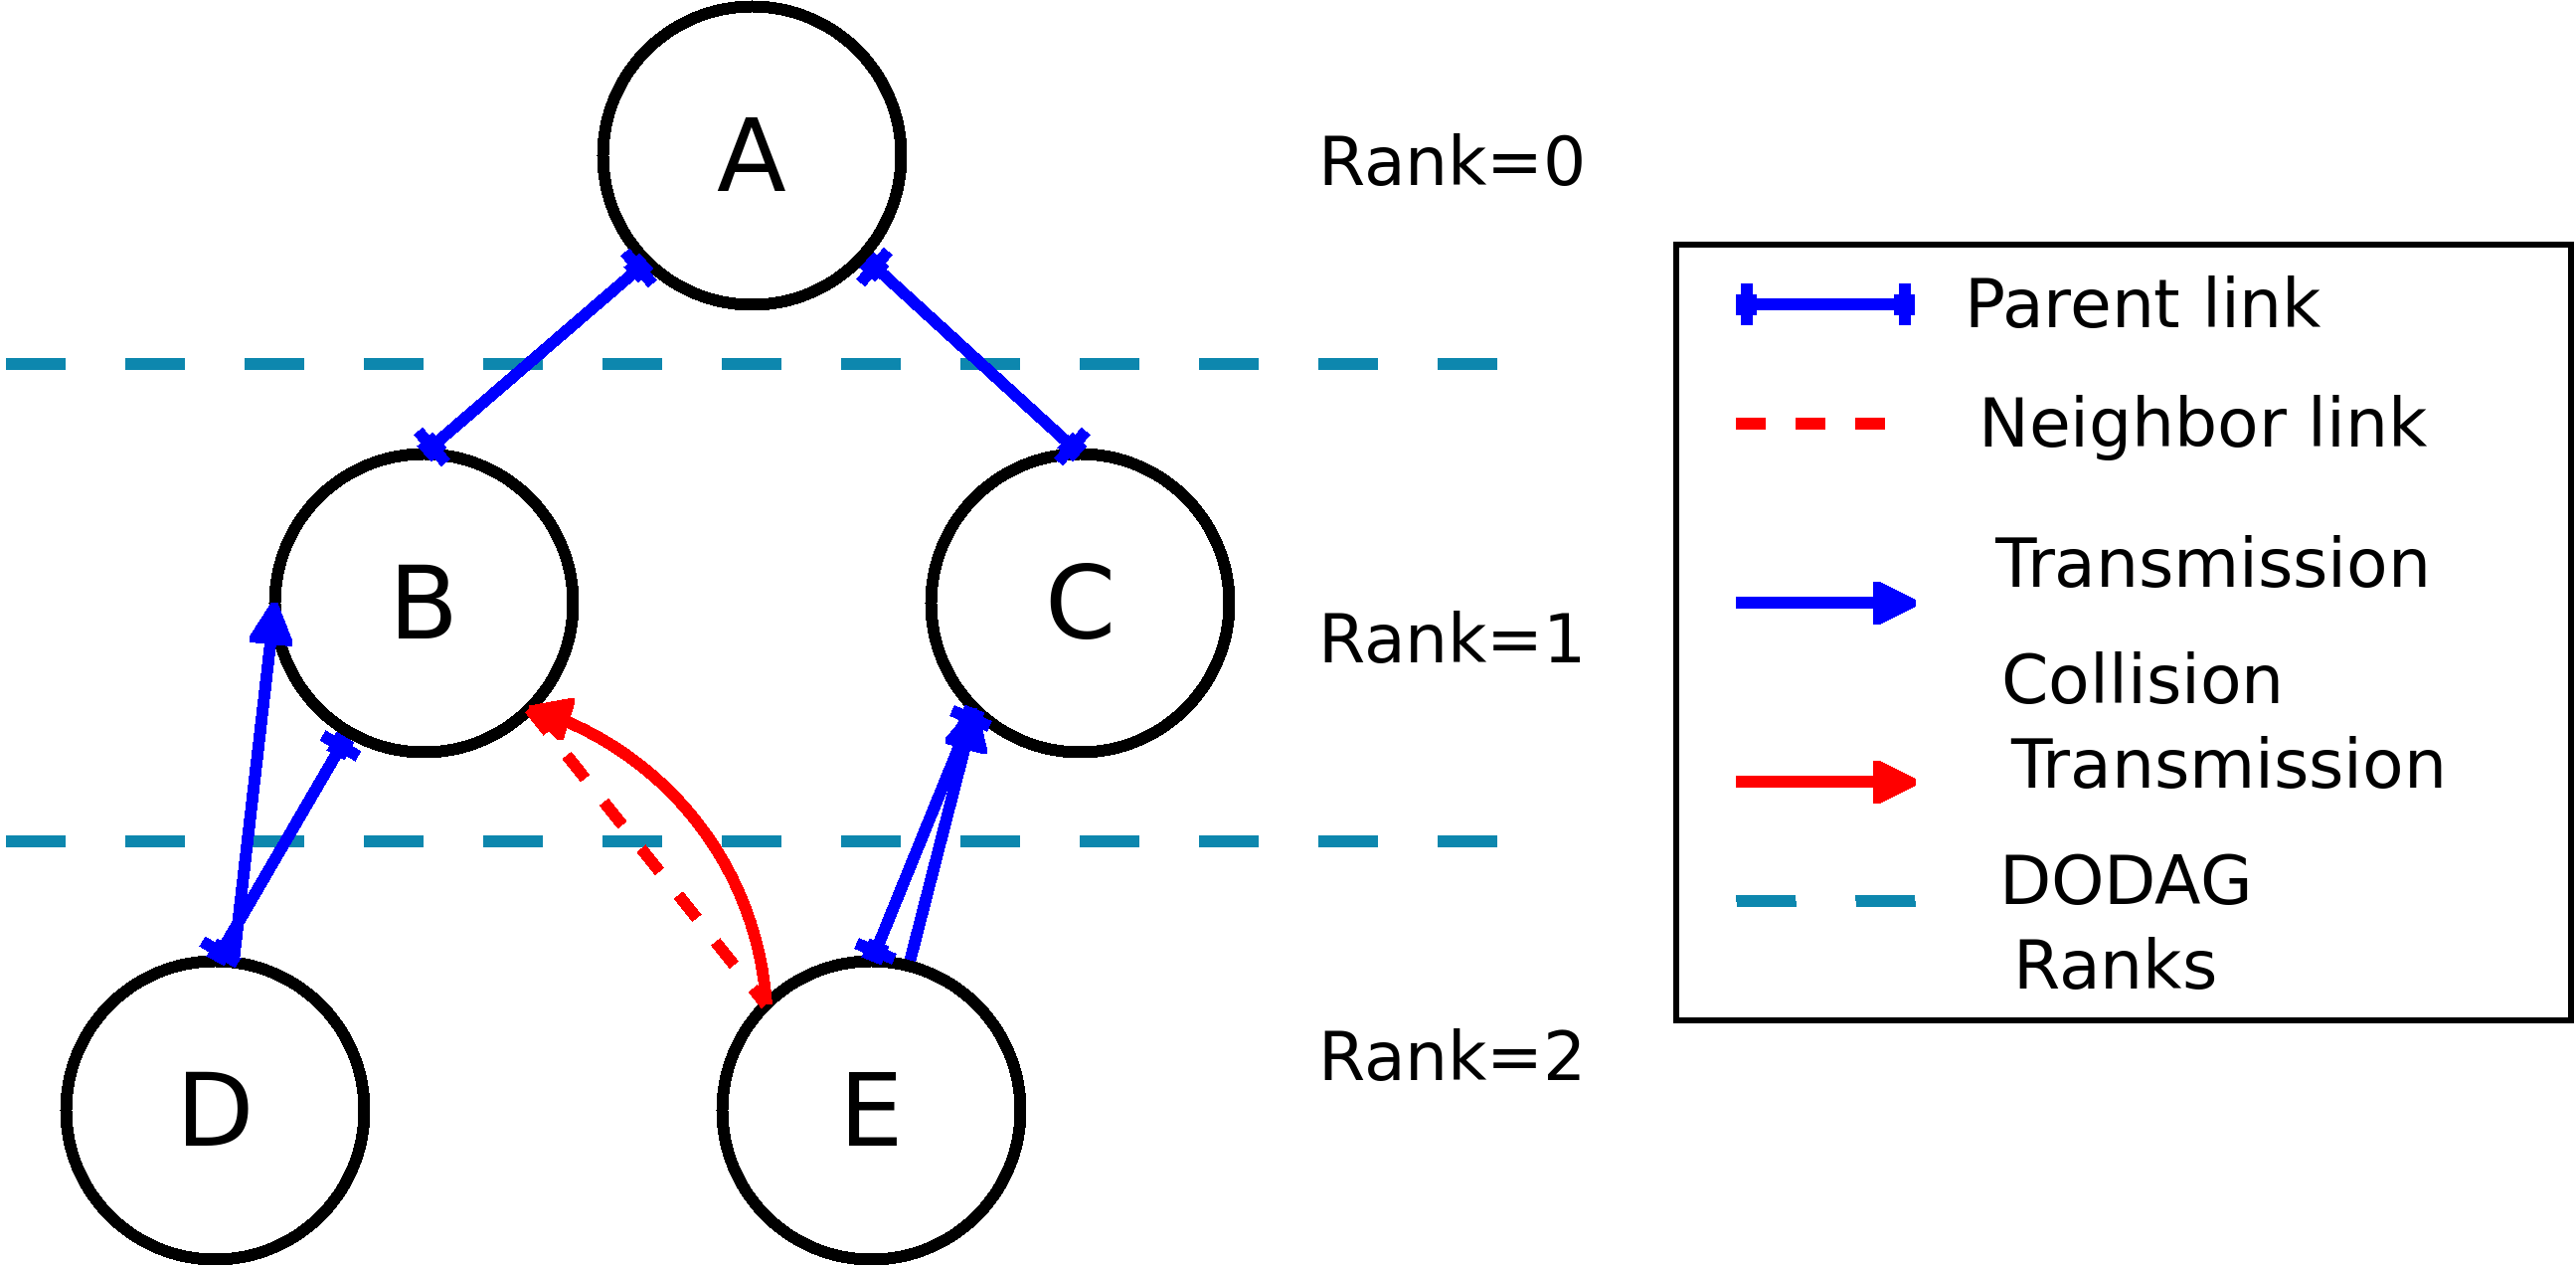
\includegraphics[width=\linewidth]{Diagram1.png}
\end{figure}
\end{minipage}
\end{frame}

\begin{frame}{Master Thesis}

\begin{block}{Proposed Mechanism}
    \begin{itemize}
    \item Local Mutual exclusion.  
    \item<2-> Using already existing transaction. 
     \item<3-> No new traffic was induced. 
      \item<4-> Achieved 70\% reduction in the colliding Tx cells. 
    \end{itemize}
    \end{block}


\centering
\begin{figure}[ht]

\item<2-> 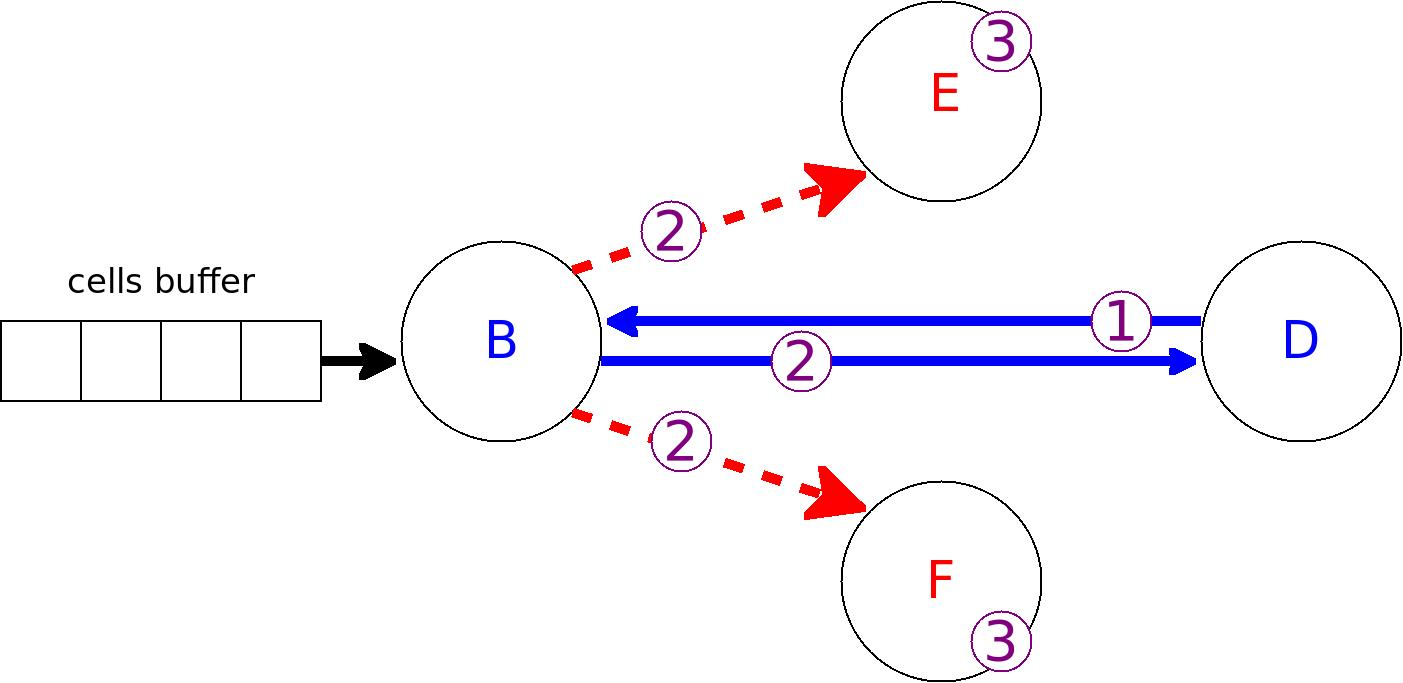
\includegraphics[width=.65\linewidth]{mech.jpeg}

\end{figure}
\end{frame}

\begin{frame}{Internship Results}


\begin{figure}[ht]


 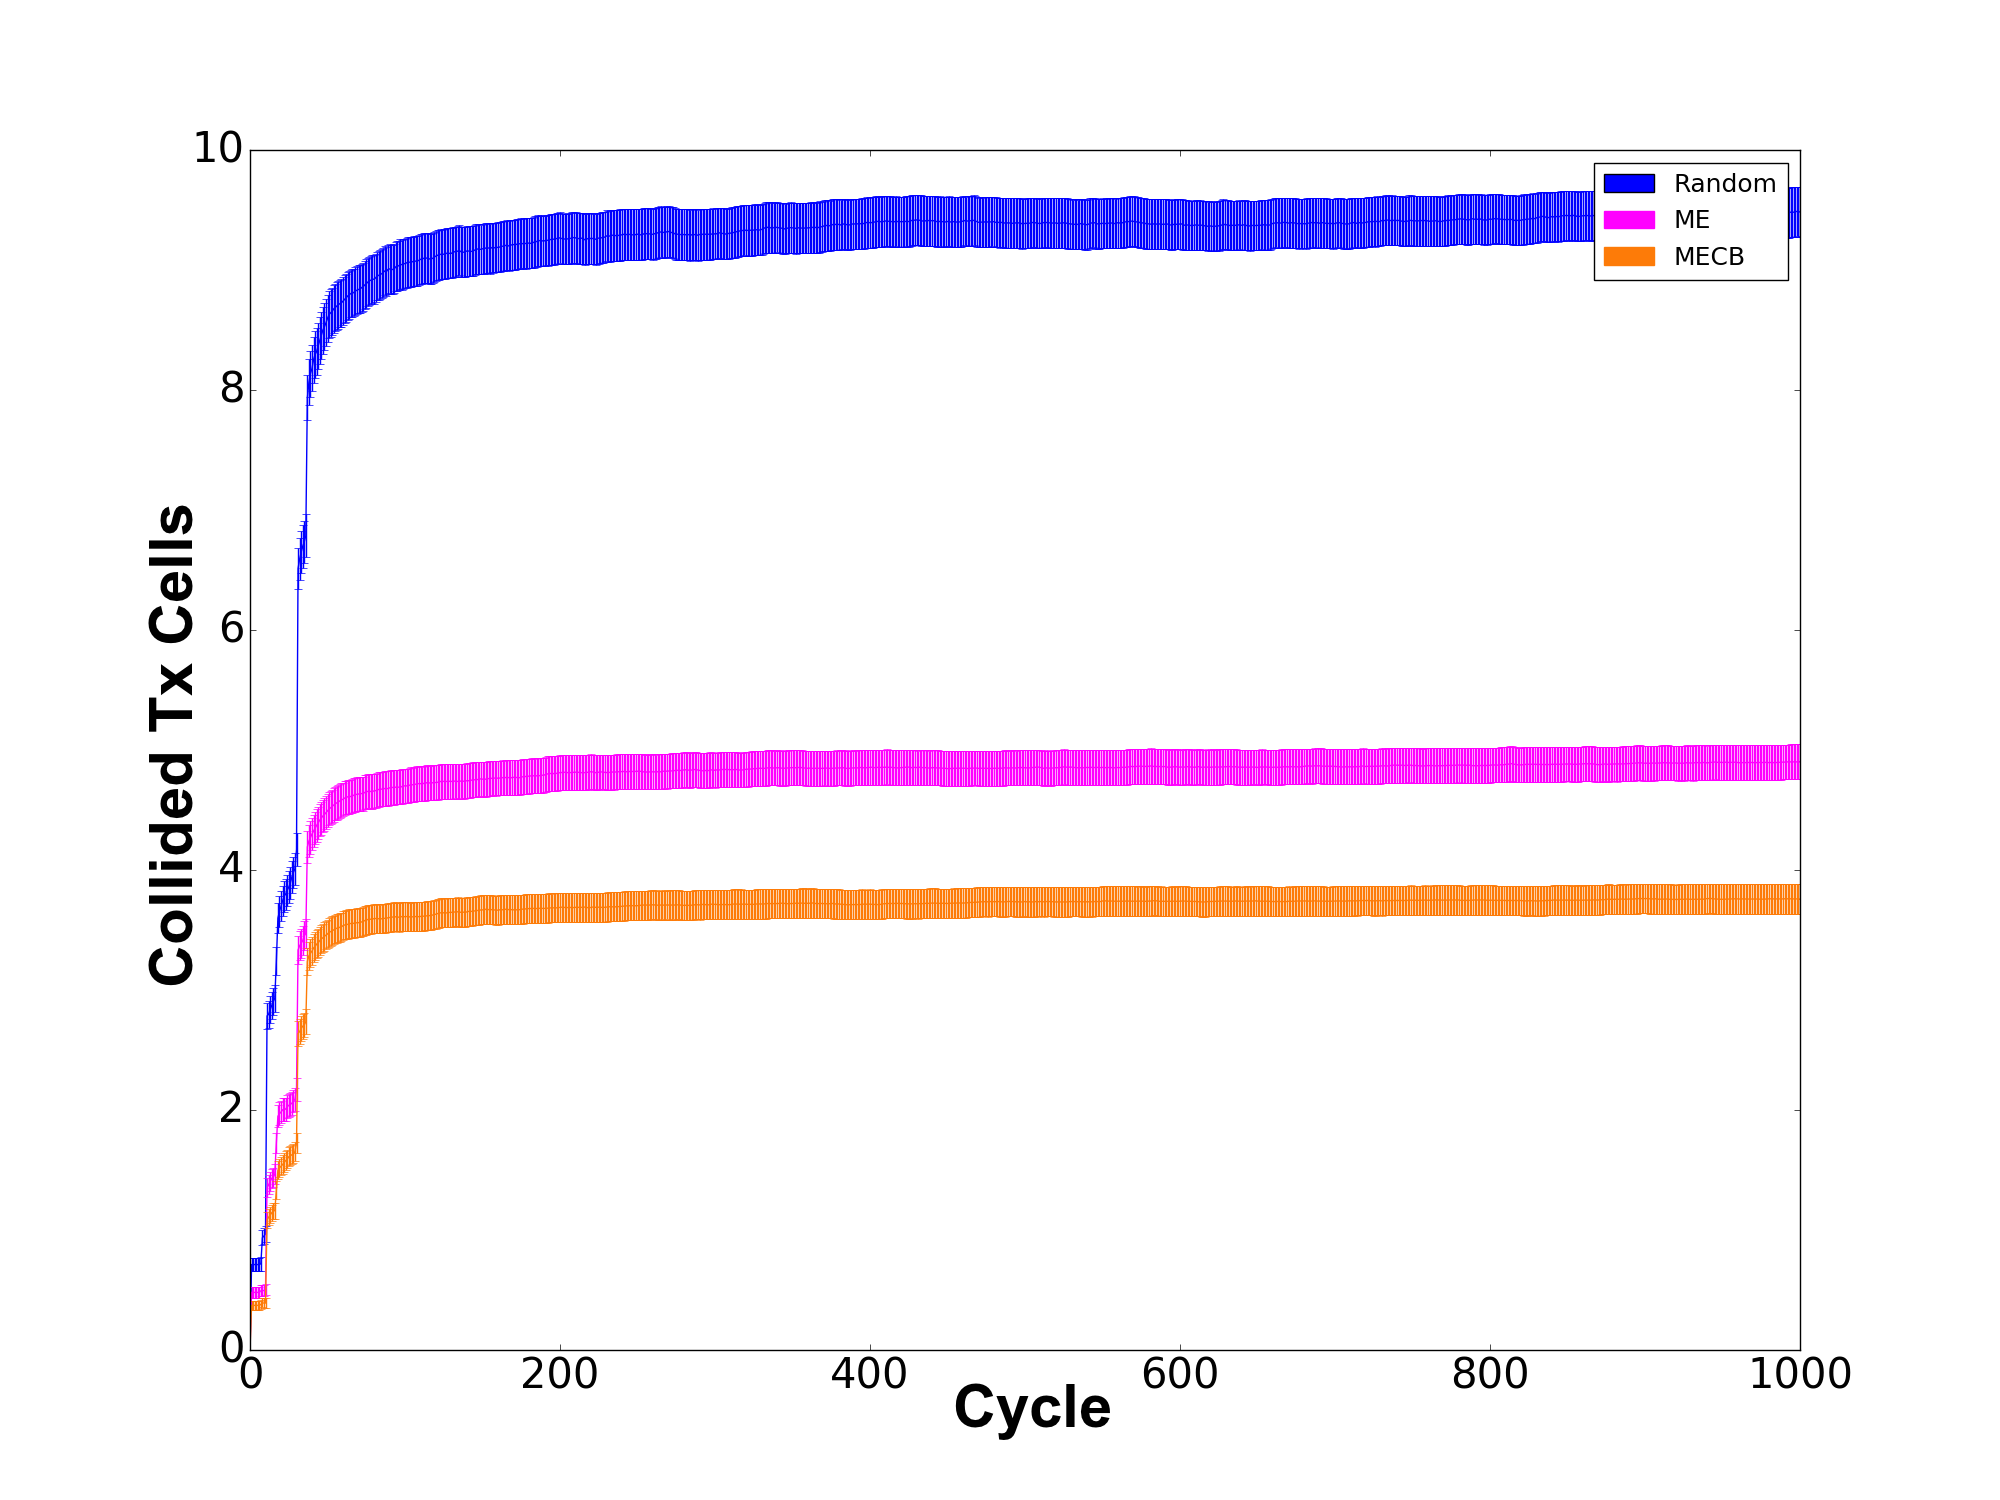
\includegraphics[width=.9\linewidth]{Graph2.png}
\end{figure}


 
\end{frame}



%%%%%%%%%%%%%%%%%%%%%%%%%%%%%%%%%%%%%%%%%%%%%%%%%%%%%
\section{State-of-the-Art for Edge Clouding}

\begin{frame}{State-of-the-Art for Edge Clouding}

\begin{block}{}
    \begin{itemize}
    \item Clouding disadvantages: latency, mobility, {\em etc}...
    \item<2->  Application-Network wall.
     \item<3-> Edge Clouding: Deploying Cloudlets in the immediate end user proximity.
      \item<4-> Using single board computers as Cloudlets
      \item<5-> Improvement of end to end latency, and application interactivity. 
      \item<6-> Current fog computing platforms remains centralized.
    \end{itemize}
    \end{block}

\end{frame}

\section{PhD Topic}
\begin{frame}{PhD Topic}
 \begin{block}{Challenges}
    \begin{itemize}
    \item Centralized control over a distributed compute/storage resources.
    \item<2-> Drawbacks of the centralized: Unnecessary traffic, latency, fragile.
    \item<3-> Implementing very large number of potentially unreliable servers.
    \item<4-> leveraging without handling the complexity of application deployment, fault tolerance, reconfiguration, or elasticity.
      
    \end{itemize}
    
    \end{block}
\end{frame}


\begin{frame}{PhD Topic}


\begin{block}{Objectives}
    \begin{itemize}
    
    \item Applying a distributed mechanism to manage the resources. 
    \item<2-> Comparing the performance of Distributed mechanisms to centralized ones. 
    \item<3-> executing cloud resource scheduling algorithms.
    \item<4-> executing gossip-based algorithms.
      
    \end{itemize}
    
    \end{block}
 \end{frame}
    
    

 

\section{Project Perspective}
\begin{frame}{Project Perspective}

    \begin{itemize}
    
    \item The importance of the topic. 
    \item<2-> Solutions using Gossip algorithms. 
    \item<3-> Advancing state-of-the-art to this hot topic. 
    
      
    \end{itemize}
    


\end{frame}


\section*{last}

\begin{frame}
\begin{tabular}{ccc}

\includegraphics[page=7, width=0.3\textwidth]{ali.pdf} &

\includegraphics[page=11, width=0.3\textwidth]{ali.pdf} &

\includegraphics[page=12, width=0.3\textwidth]{ali.pdf} \\


\includegraphics[page=18, width=0.3\textwidth]{ali.pdf} &

\includegraphics[page=26, width=0.3\textwidth]{ali.pdf} &

\includegraphics[page=29, width=0.3\textwidth]{ali.pdf} \\




\end{tabular}

\begin{block}{}
\centering Thanks for your attention!\\
Questions?
\end{block}
\end{frame}










\end{document}


